\documentclass[crop,tikz]{standalone}
\usepackage{tikz}
\usepackage{amsmath}
\usetikzlibrary{arrows}

%\usetikzlibrary {decorations.pathmorphing}
\begin{document}

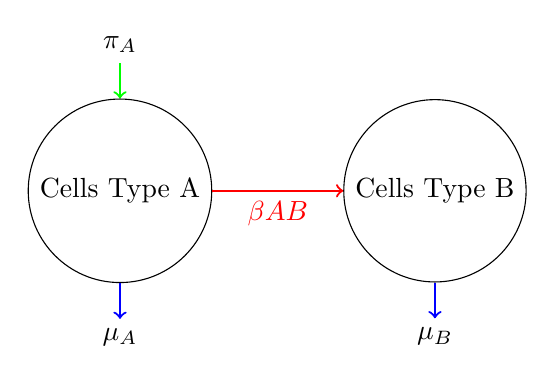
\begin{tikzpicture}
	\path (0,1) node[circle,draw,pin={[pin edge={<-,thick,green}]above:$\pi_A$},pin={[pin edge={->,thick,blue}]below:$\mu_A$}]  (x) {Cells Type A}
	(4,1) node[circle,draw,pin={[pin edge={->,thick,blue}]below:$\mu_B$}](y) {Cells Type B};
%	\draw[->,blue]  (x) -- (y);
	\draw[->,red,thick]    (x) -- node[below] {$\beta A B$} (y);
%	\draw[->,orange] (x) .. controls +(up:1cm) and +(left:1cm) .. node[above,sloped] {label} (y);
\end{tikzpicture}



\end{document}